\newpage
\section{Review the predictor variables and guess what their role in a credit decision might be. Are there any surprises in the data?} \label{appendix1}
As follows the data set is being explored in four steps. First of all we will look into the dependent variable $RESPONSE$ (see figure \ref{response}) and then all categorical variables (see figure \ref{categoricals}) excluding the $ OBS\#$ variable will be explored. Following this we will look at all numerical variables (see figure \ref{scatterplot}) and finally a correlation matrix as well as statistical overview of all variables will be conducted (see figure \ref{corrMatrix} and \ref{overview} respectively). The German Credit data set contains n=1.000 observations with 300 responses with bad credit rating and 700 responses with good credit rating.\\ %Hier müsste man eigtl. in Frage stellen, ob dieses Datenset der Regeln von Zufall entspricht.
\begin{figure}[htbp]
	\centering
	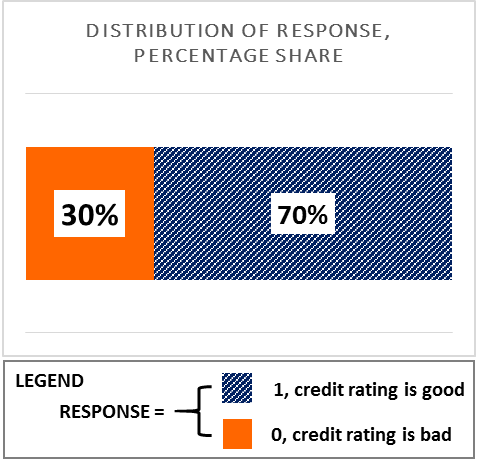
\includegraphics[width=0.4\textwidth]{response.png}
	\caption{Distribution of $RESPONSE$, percentage share, n=1.000 observations}
	\label{response}
\end{figure}\\
In figure \ref{categoricals} we can see the distribution of $RESPONSE$ by all other categorical variables $CHECK\_ACC$, $HISTORY$, $SAV\_ACCT$, $PRESENT\_RESIDENT$, $EMPLOYMENT$, and $JOB$. According to \cite[pp.76-77]{shmueli} categorical variables can inflate the dimension of the dataset which we can see by comparing the original dataset which had 20 variables in total and the preprocessed data set which has 32 variables (due to categorical and binary variables). The preprocessing however is necessary in order to be able to conduct data mining methods on the data set. \cite[pp.76-77]{shmueli} suggest to reduce the number of sub-categories through combination of similar sub-categories. 

Regarding the distribution of $RESPONSE$ by $CHECK\_ACC$ there are four sub-categories with each having different distributions so that combining categories would not be a good choice. Sub-category \textit{0:< 0 DM} is the worst and sub-category \textit{3:no checking account} is the best according to the given data set. Putting the attribute \textit{3:no checking account} as best outcome is strange because if there is no checking account then for instance a bank does not have any business and therefore it is actually a rather bad attribute. Since we do not have domain knowledge the order of $CHECK\_ACC$ will be kept as it is.

Looking at the distribution of $RESPONSE$ by $HISTORY$ there are five sub-categories with categories \textit{0:no credits taken} and \textit{1:all credits at this bank paid back} as well as \textit{2:existing credits paid back duly} and \textit{3:delay in paying off in the past} having similar distributions. With respect to their similarities in distribution these two pairs of categories could be combined, however with regard to the rather different attributional message of these variables as well as the missing domain knowledge, these variables are not combined. Regardless of this the order has to be reversed to stay constistent with $CHECK\_ACC$ (and for the interpretation) because the worst attribute is assigned the best category at the moment. With regard to $SAV\_ACCT$ there is the same issue as with $HISTORY$. Here two categories \textit{0:< 100 DM} and \textit{1:100$\leq$..<500 DM} can be combined as well as the three other categories. However since each sub-category describes different attributions and due to missing domain knowledge the order will be kept as it is. 

Regarding $PRESENT\_RESIDENT$ all four sub-categories have a similar distribution which leads to the assumption that they could be combined. However combining these categories would create a non-sense category. Furthermore there is an error in the data set regarding this variable with respect to the inconsistency of the coding which starts at 0 and ends with 3. The raw data set however starts with the value 1 and ends with the value 4. We could assume that during the transformation process the values were shiftet by 1 unit. Since it is not retraceable how the error occured we decide to omitt this variable for the later analysis.

The variable $EMPLOYMENT$ is sub-divided into five sub-categories with each having a slightly different distribution. We decide not to combine categories in this category because a long employment status implies higher income security and thus it makes sense to leave the categories as they are.

Finally the variable $JOB$ is sub-divided into four sub-categories with each having a slightly different distribution. Sub-category \textit{0:unemployed/unskilled - non-resident} is surprising because an unskilled nature of the job is sub-divided wether its an resident or not with non-residence being worse. The categories as they currently are in the right ascending order and due to their individual attributional message should remain in different categories. 
\begin{figure}[htbp]
	\centering
	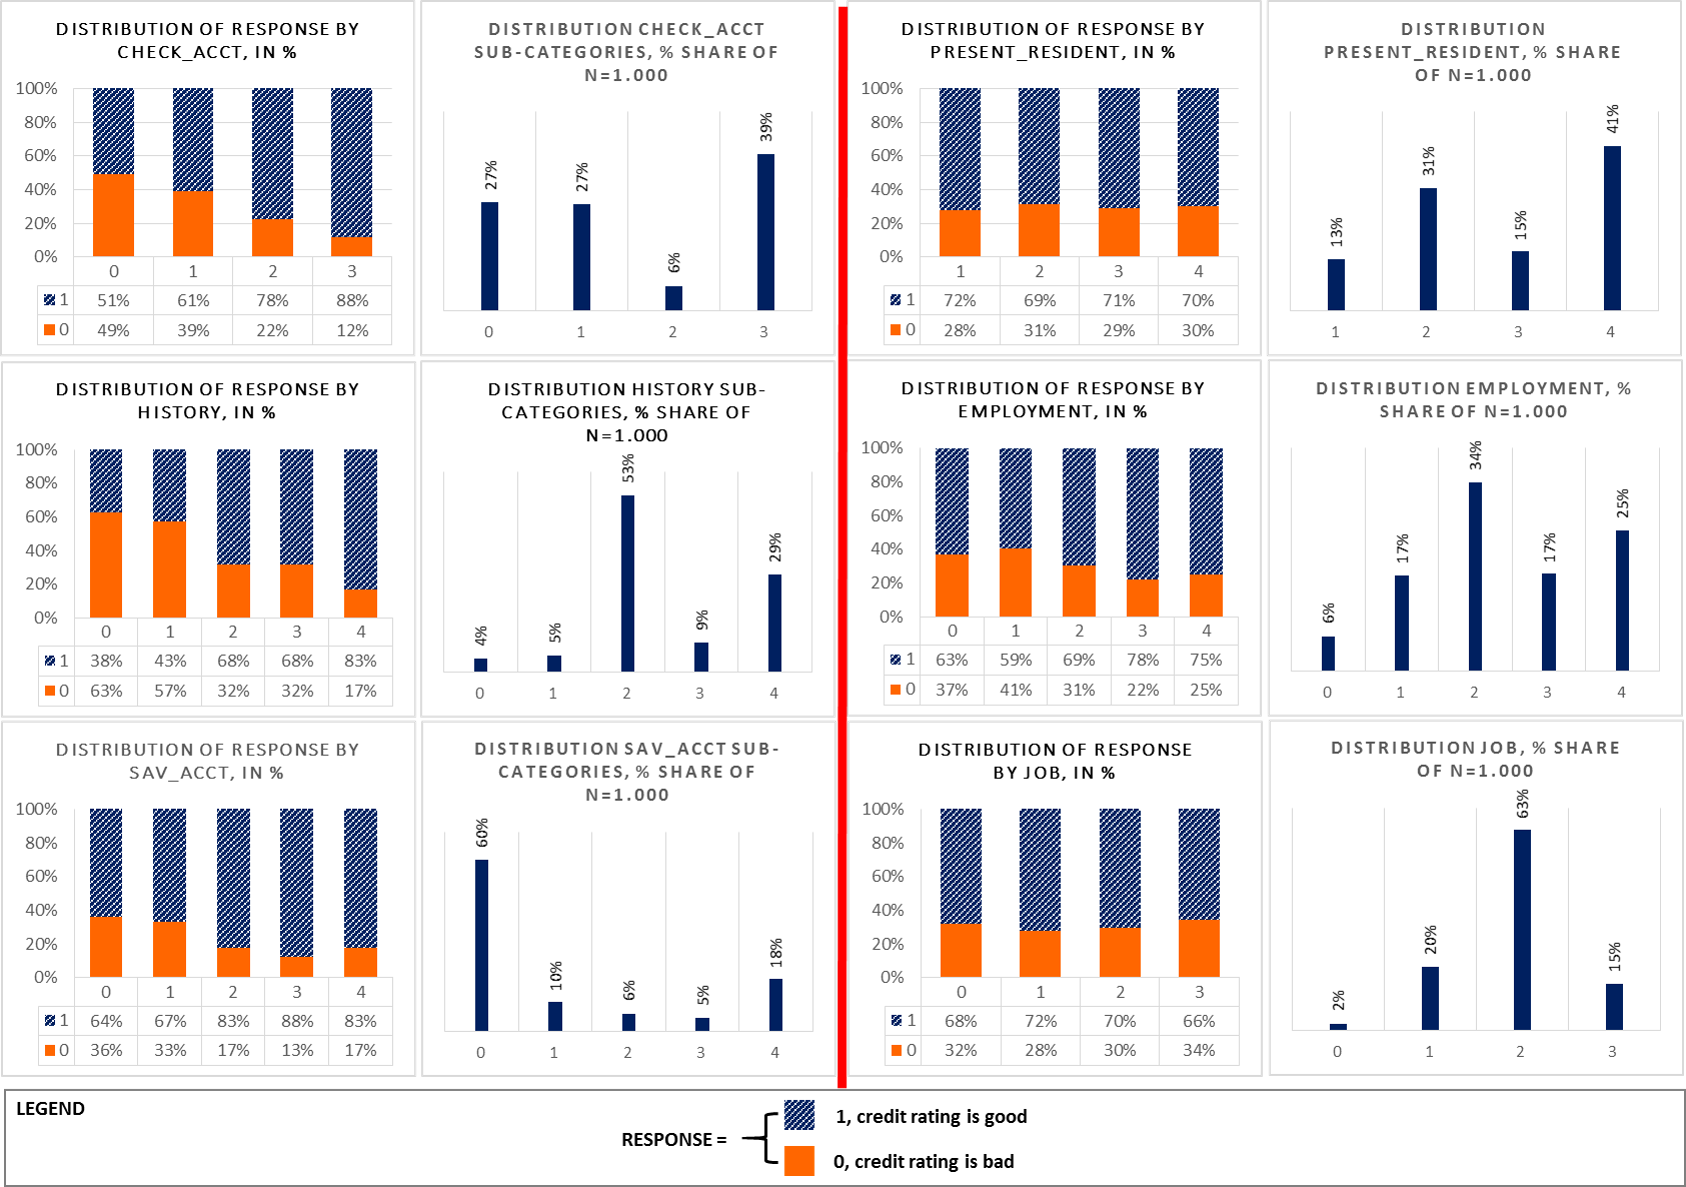
\includegraphics[width=0.7\textwidth]{categoricals.png}
	\caption{Distribution of $RESPONSE$ with other Categorical variables, percentage share of sub-categories of each category, n=1.000}
	\label{categoricals}
\end{figure}\\
Figure \ref{scatterplot} displays all numerical pairwise scatterplots: $DURATION$, $AMOUNT$, $INSTALL\_RATE$, $AGE$, $NUM\_CREDITS$, and $NUM\_DEPENDENT$. According to the scatterplot there is a positive correlation between $DURATION$ and $AMOUNT$. Other correlations, where the trend is not clear, are between $DURATION$ and $AGE$ as well as $AMOUNT$ and $AGE$. From the only few numbers and thus resulting patterns of the other variables $INSTALL\_RATE$, $NUM\_CREDITS$, and $NUM\_DEPENDENT$ on can conclude that these variables are not numerical in nature. %Man müsste doch eigtl. hier auch Rückschlüsse ziehen können ob da auch einfach kein Zusammenhang ist....
\begin{figure}[htbp!]
	\centering
	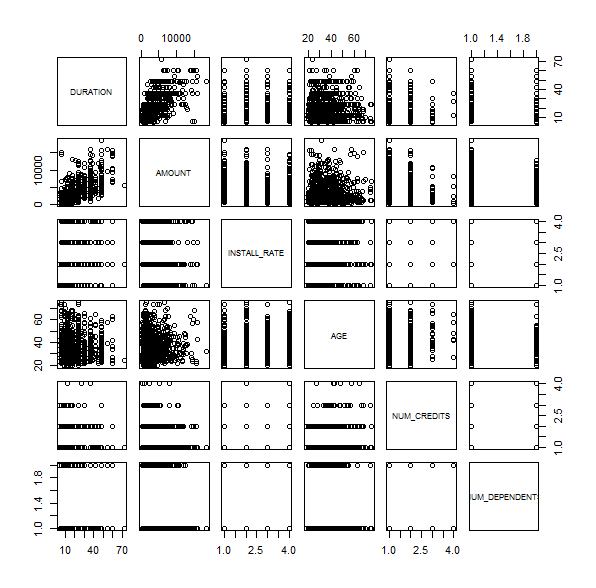
\includegraphics[width=\textwidth]{scatterplot.png}
	\caption{Scatterplot Matrix of Numerical Variables, n=1.000}
	\label{scatterplot}
\end{figure}\\
In figure \ref{corrMatrix} the correlation matrix of the German Credit data set is displayed. According to the correlation matrix there is one pair of variables which has a high correlation coefficient of -0.74\footnote{A high correlation coefficient is set in this analysis when the coefficient is $\geq$ |0.7|}. This implies that there is multicollinearity regarding this pair.
\begin{figure}[htbp]
	\centering
	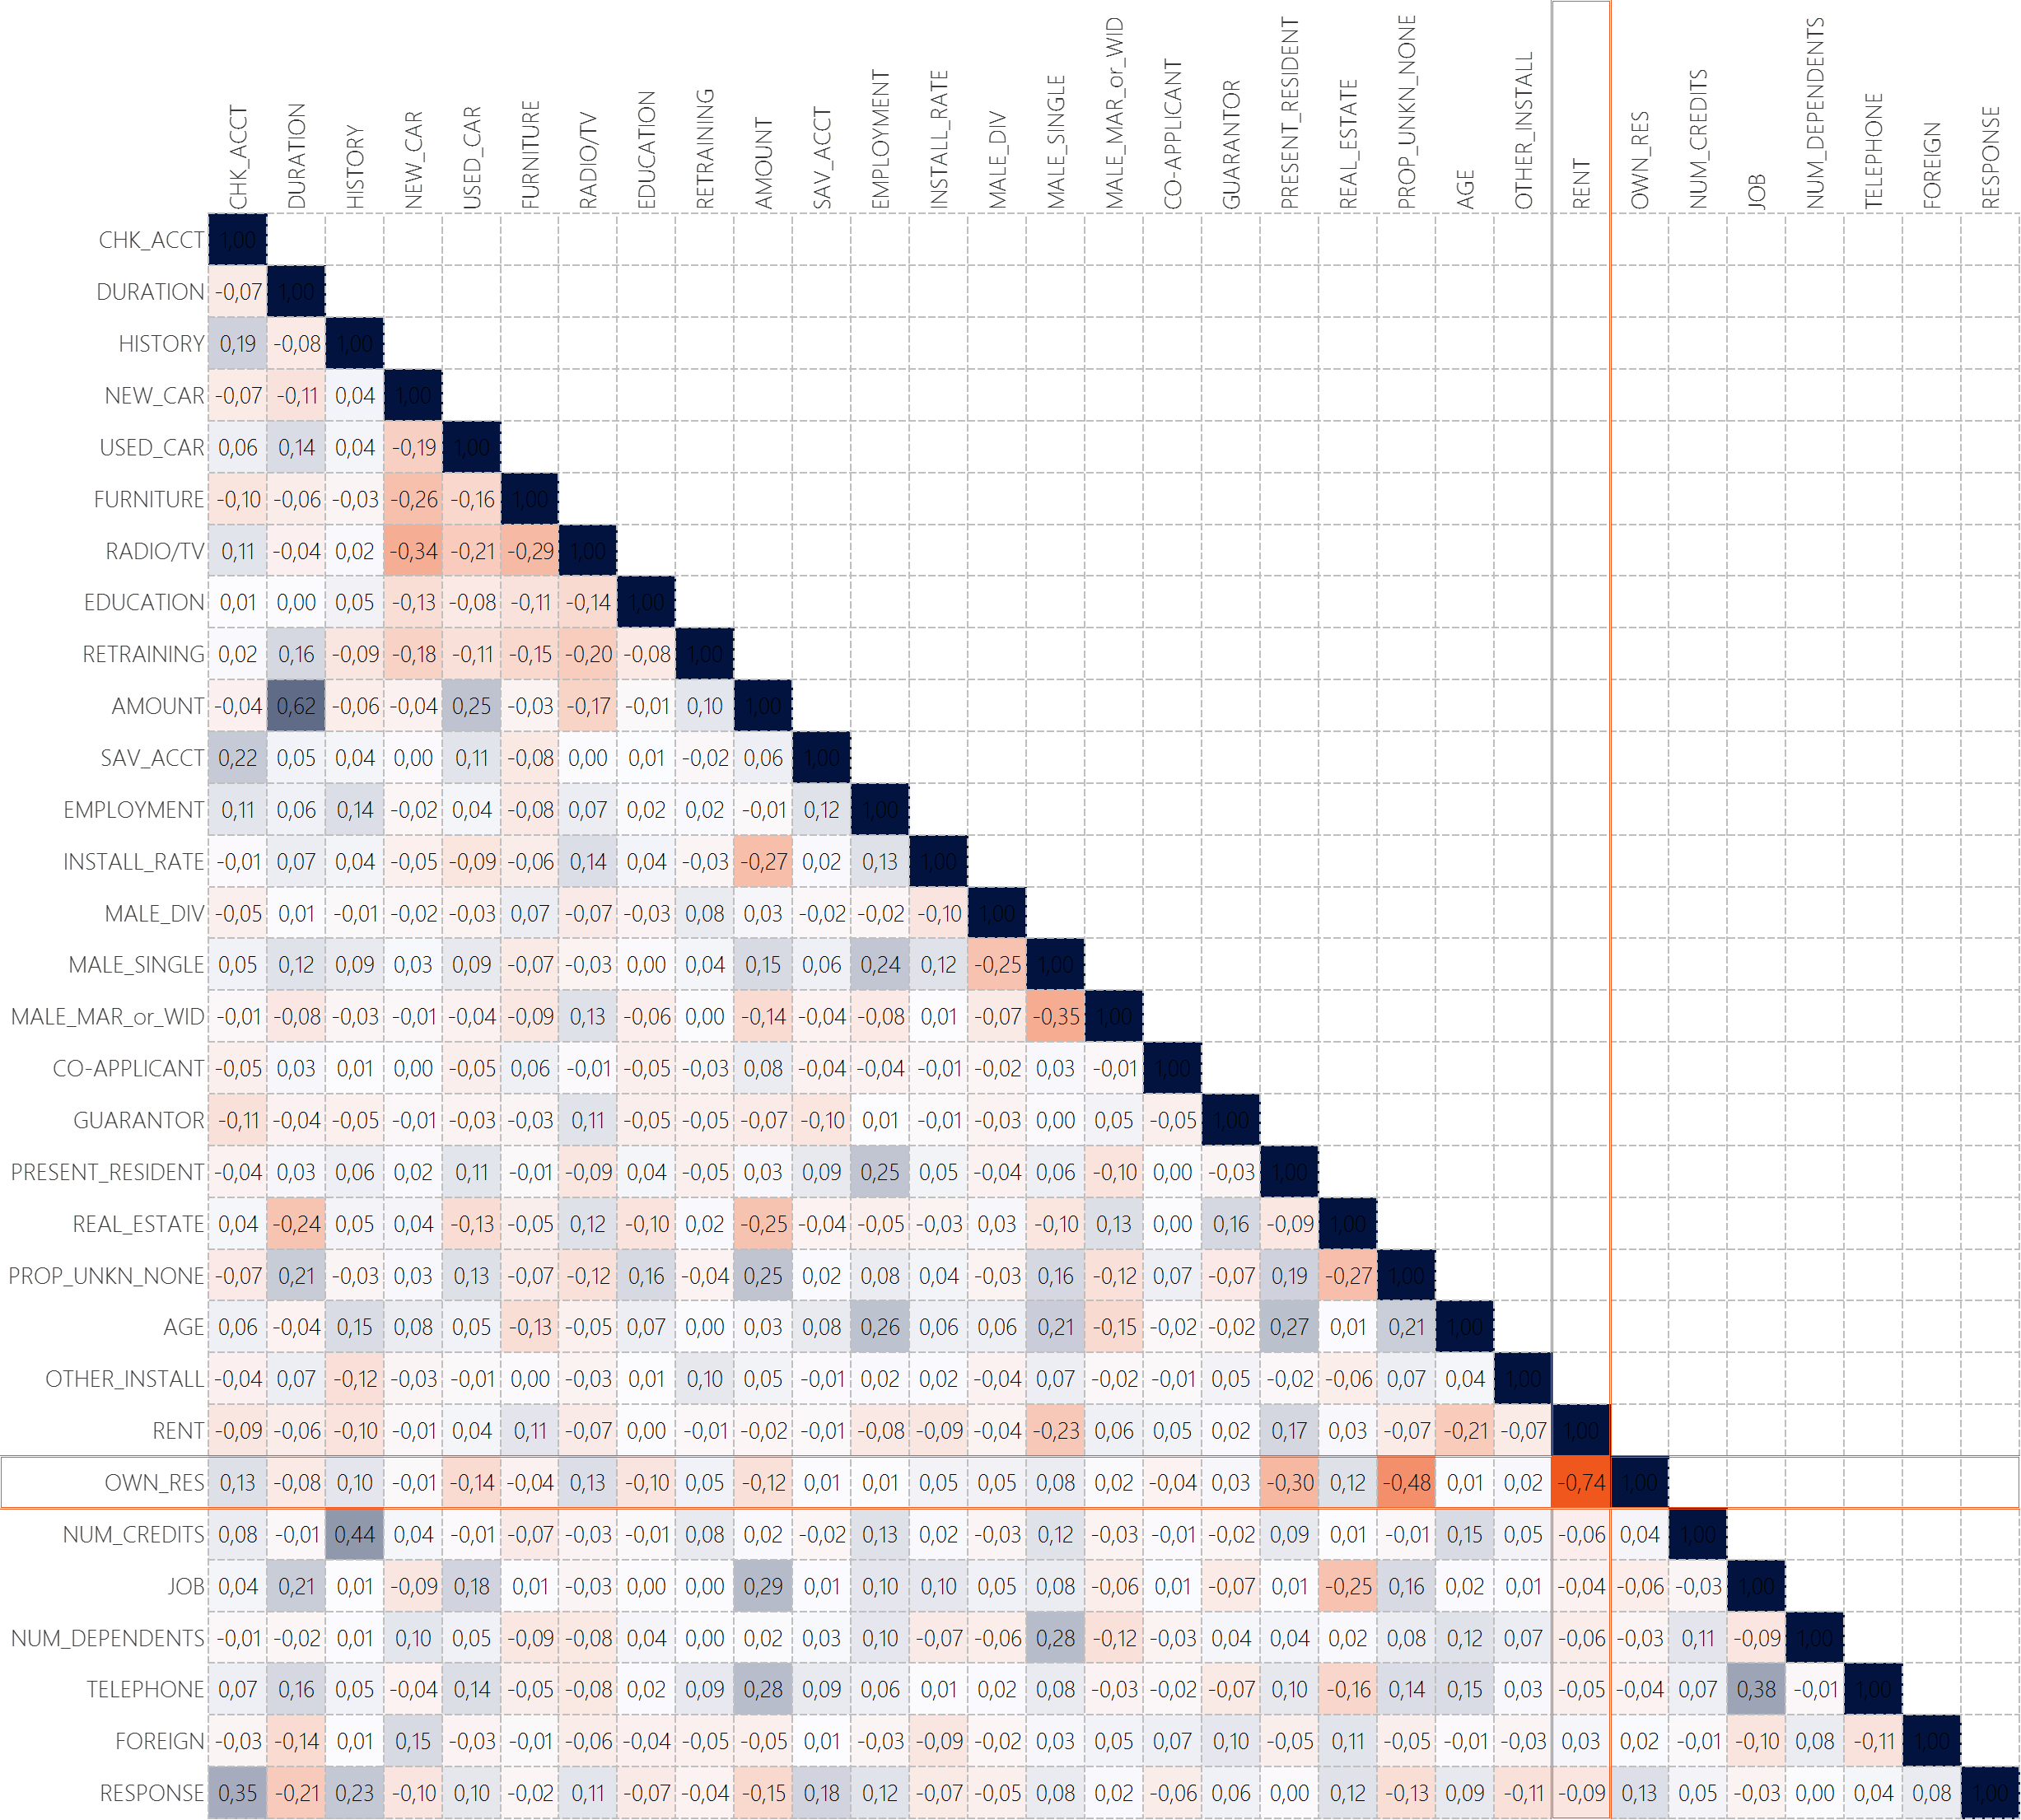
\includegraphics[width=\textwidth]{CorrPlot.png}
	\caption{Correlation Matrix of German Credit Data Set, n=1.000}
	\label{corrMatrix}
\end{figure}\\
Finally table \ref{overview} provides an overview about basic statistical values for all variables. We can see that there is a great variety in terms of the variables' range which has to be taken into consideration. %Irgendwas wegen der skewness sagen
\begin{table}[]
	\centering
	\caption{Statistical Overview of German Credit Data Set, n=1.000}
	\label{overview}
	\begin{tabular}{|p{2.6cm}|p{0.75cm}|p{0.6cm}|p{0.75cm}|p{0.6cm}|p{0.75cm}|p{1.2cm}|p{0.6cm}|p{0.65cm}|p{0.7cm}|p{0.45cm}|p{0.65cm}|p{0.85cm}|p{0.55cm}|}\hline
		{\tiny \textbf{Variable}}
		&{\tiny \textbf{Av. Value}}&{\tiny \textbf{SE}}&{\tiny \textbf{Med.}}&\textbf{{\tiny Mod.}} &\textbf{$\sigma$}&\textbf{{\tiny Sample }}$\sigma^2$&{\tiny\textbf{Curto- sis}}&
		{\tiny\textbf{Skew- ness}}
		&{\tiny \textbf{Value Range}}&{\tiny \textbf{Min.}}&{\tiny \textbf{Max.}}&{\tiny \textbf{Sum}}
		&\textbf{{\tiny Conf. lvl}}\\\hline
		{\tiny OBS\#}
		&{\tiny 500,50}&{\tiny 9,13}&{\tiny 500,50}&{\tiny \#N/A}
		&{\tiny 288,82}&{\tiny 83.416,67}&{\tiny (1,20)}&{\tiny (0,00)}
		&{\tiny 999}&{\tiny 1}&{\tiny 500.500}&{\tiny 1.000}&{\tiny 17,92}\\ \hline
		{\tiny CHK\_ACCT}
		&{\tiny 1,58}&{\tiny 0,04}&{\tiny 1,00}&{\tiny 3}
		&{\tiny 1,26}&{\tiny 1,58}&{\tiny (1,66)}&{\tiny 0,01}
		&{\tiny 3}&{\tiny - }&{\tiny 3}&{\tiny 1.577}&{\tiny 0,08}\\ \hline
		{\tiny DURATION}
		&{\tiny 20,90}&{\tiny 0,38}&{\tiny 18,00}&{\tiny 24}
		&{\tiny 12,06}&{\tiny 145,42}&{\tiny 0,92}&{\tiny 1,09}
		&{\tiny 68}&{\tiny 4}&{\tiny 72}&{\tiny 20.903}&{\tiny 0,75}\\ \hline
		{\tiny HISTORY}
		&{\tiny 2,55}&{\tiny 0,03}&{\tiny 2,00}&{\tiny 2}
		&{\tiny 1,08}&{\tiny 1,17}&{\tiny (0,58)}&{\tiny (0,01)}
		&{\tiny 4}&{\tiny -}&{\tiny 4}&{\tiny 2.545}&{\tiny 0,07}\\ \hline
		{\tiny NEW\_CAR}
		&{\tiny 0,23}&{\tiny 0,01}&{\tiny -}&{\tiny -}
		&{\tiny 0,42}&{\tiny 0,18}&{\tiny (0,42)}&{\tiny 1,26}
		&{\tiny 1}&{\tiny -}&{\tiny 1}&{\tiny 234}&{\tiny 0,03}\\ \hline
		{\tiny USED\_CAR}
		&{\tiny 0,10}&{\tiny 0,01}&{\tiny -}&{\tiny -}
		&{\tiny 0,30}&{\tiny 0,09}&{\tiny 4,85}&{\tiny 2,62}
		&{\tiny 1}&{\tiny -}&{\tiny 1}&{\tiny 103}&{\tiny 0,02}\\ \hline
		{\tiny FURNITURE}
		&{\tiny 0,18}&{\tiny 0,01}&{\tiny -}&{\tiny -}
		&{\tiny 0,39}&{\tiny 0,15}&{\tiny 0,76}&{\tiny 1,66}
		&{\tiny 1}&{\tiny -}&{\tiny 1}&{\tiny 181}&{\tiny 0,02}\\ \hline
		{\tiny RADIO/TV}
		&{\tiny 0,28}&{\tiny 0,01}&{\tiny -}&{\tiny -}
		&{\tiny 0,45}&{\tiny 0,20}&{\tiny (1,04)}&{\tiny 0,98}
		&{\tiny 1}&{\tiny -}&{\tiny 1}&{\tiny 280}&{\tiny 0,03}\\ \hline
		{\tiny EDUCATION}
		&{\tiny 0,05}&{\tiny 0,01}&{\tiny -}&{\tiny -}
		&{\tiny 0,22}&{\tiny 0,05}&{\tiny 15,13}&{\tiny 4,14}
		&{\tiny 1}&{\tiny -}&{\tiny 1}&{\tiny 50}&{\tiny 0,01}\\ \hline
		{\tiny RETRAINING}
		&{\tiny 0,10}&{\tiny 0,01}&{\tiny -}&{\tiny -}
		&{\tiny 0,30}&{\tiny 0,09}&{\tiny 5,45}&{\tiny 2,73}
		&{\tiny 1}&{\tiny -}&{\tiny 1}&{\tiny 97}&{\tiny 0,02}\\ \hline
		{\tiny AMOUNT}
		&{\tiny  3.271,26}&{\tiny 89,26}&{\tiny 2.319,50}&{\tiny 1.393}
		&{\tiny 2.822,74}&{\tiny 7.967.843,47}&{\tiny 4,29}&{\tiny 1,95}
		&{\tiny 18.174}&{\tiny 250}&{\tiny 18.424}&{\tiny 3.271.258}&{\tiny 175,16}\\ \hline
		{\tiny SAV\_ACCT}
		&{\tiny 1,11}&{\tiny 0,05}&{\tiny -}&{\tiny -}
		&{\tiny 1,58}&{\tiny 2,50}&{\tiny (0,68)}&{\tiny 1,02}
		&{\tiny 4}&{\tiny -}&{\tiny 4}&{\tiny 1.105}&{\tiny 0,10}\\ \hline
		{\tiny EMPLOYMENT}
		&{\tiny 2,38}&{\tiny 0,04}&{\tiny 2,00}&{\tiny 2}
		&{\tiny 1,21}&{\tiny 1,46}&{\tiny (0,93)}&{\tiny (0,12)}
		&{\tiny 4}&{\tiny -}&{\tiny 4}&{\tiny 2.384}&{\tiny 0,07 }\\ \hline
		{\tiny INSTALL\_RATE}
		&{\tiny 2,97}&{\tiny 0,04}&{\tiny 3,00}&{\tiny 4}
		&{\tiny 1,12}&{\tiny 1,25}&{\tiny (1,21)}&{\tiny (0,53)}
		&{\tiny 3}&{\tiny 1}&{\tiny 4}&{\tiny 2.973}&{\tiny 0,07}\\ \hline
		{\tiny MALE\_DIV}
		&{\tiny 0,05}&{\tiny 0,01}&{\tiny -}&{\tiny -}
		&{\tiny 0,22}&{\tiny 0,05}&{\tiny 15,13}&{\tiny 4,14}
		&{\tiny 1}&{\tiny -}&{\tiny 1}&{\tiny 50}&{\tiny 0,01}\\ \hline
		{\tiny MALE\_SINGLE}
		&{\tiny 0,55}&{\tiny 0,02}&{\tiny 1,00}&{\tiny 1}
		&{\tiny 0,50}&{\tiny 0,25}&{\tiny (1,97)}&{\tiny (0,19)}
		&{\tiny 1}&{\tiny -}&{\tiny 1}&{\tiny 548}&{\tiny 0,03}\\ \hline
	    {\tiny 	MALE\_MAR\_or\_WID}
	    &{\tiny 0,09}&{\tiny 0,01}&{\tiny -}&{\tiny -}
	    &{\tiny 0,29}&{\tiny 0,08}&{\tiny 6,01}&{\tiny 2,83}
	    &{\tiny 1}&{\tiny -}&{\tiny 1}&{\tiny 92}&{\tiny 0,02}\\ \hline
		{\tiny CO-APPLICANT}
		&{\tiny 0,04}&{\tiny 0,01}&{\tiny -}&{\tiny -}
		&{\tiny 0,20}&{\tiny 0,04}&{\tiny 19,54}&{\tiny 4,64}
		&{\tiny }&{\tiny -}&{\tiny 1}&{\tiny 41}&{\tiny 0,01}\\ \hline
		{\tiny GUARANTOR}
		&{\tiny 0,05}&{\tiny 0,01}&{\tiny -}&{\tiny -}
		&{\tiny 0,22}&{\tiny 0,05}&{\tiny 14,36}&{\tiny 4,04}
	    &{\tiny 1}&{\tiny -}&{\tiny 1}&{\tiny 52}&{\tiny 0,01}\\ \hline
		{\tiny PRESENT\_RESIDENT}
		&{\tiny 2,85}&{\tiny 0,03}&{\tiny 3,00}&{\tiny 4}
		&{\tiny 1,10}&{\tiny 1,22}&{\tiny (1,38)}&{\tiny (0,27)}
		&{\tiny 3}&{\tiny 1}&{\tiny 4}&{\tiny 2.845}&{\tiny 0,07}\\ \hline
		{\tiny REAL\_ESTATE}
		&{\tiny 0,28}&{\tiny 0,01}&{\tiny -}&{\tiny -}
		&{\tiny 0,45}&{\tiny 0,20}&{\tiny (1,06)}&{\tiny 0,97}
		&{\tiny 1}&{\tiny -}&{\tiny 1}&{\tiny 282}& {\tiny 0,03}\\ \hline
		{\tiny PROP\_UNKN\_NONE}
		&{\tiny 0,15}&{\tiny 0,01}&{\tiny -}&{\tiny -}
		&{\tiny 0,36}&{\tiny 0,13}&{\tiny 1,69}&{\tiny 1,92}
		&{\tiny 1}&{\tiny -}&{\tiny 1}&{\tiny 154}&{\tiny 0,02}\\ \hline
		{\tiny AGE}
		&{\tiny 35,55}&{\tiny 0,36}&{\tiny 33,00}&{\tiny 27}
		&{\tiny 11,38}&{\tiny 129,40}&{\tiny 0,60}&{\tiny 1,02}
		&{\tiny 56}&{\tiny 19}&{\tiny 75}&{\tiny 35.546}&{\tiny 0,71}\\ \hline
		{\tiny OTHER\_INSTALL}
		&{\tiny 0,19}&{\tiny 0,01}&{\tiny -}&{\tiny -}
		&{\tiny 0,39}&{\tiny 0,15}&{\tiny 0,61}&{\tiny 1,62}
		&{\tiny 1}&{\tiny -}&{\tiny 1}&{\tiny 186}&{\tiny 0,02}\\ \hline
		{\tiny RENT}
		&{\tiny 0,18}&{\tiny 0,01}&{\tiny -}&{\tiny -}
		&{\tiny 0,38}&{\tiny 0,15}&{\tiny 0,81}&{\tiny 1,68}
		&{\tiny 1}&{\tiny -}&{\tiny 1}&{\tiny 179}&{\tiny 0,02}\\ \hline
		{\tiny OWN\_RES}
		&{\tiny 0,71}&{\tiny 0,01}&{\tiny 1,00}&{\tiny 1}
		&{\tiny 0,45}&{\tiny 0,20}&{\tiny (1,11)}&{\tiny (0,94)}
		&{\tiny 1}&{\tiny -}&{\tiny 1}&{\tiny 713}&{\tiny 0,03}\\ \hline
		{\tiny NUM\_CREDITS}
		&{\tiny 1,41}&{\tiny 0,02}&{\tiny 1,00}&{\tiny 1}
		&{\tiny 0,58}&{\tiny 0,33}&{\tiny 1,60}&{\tiny 1,27}&
		{\tiny 3}&{\tiny 1}&{\tiny 4}&{\tiny 1.407}&{\tiny 0,04}\\ \hline
		{\tiny JOB}
		&{\tiny 1,90}&{\tiny 0,02}&{\tiny 2,00}&{\tiny 2}
		&{\tiny 0,65}&{\tiny 0,43}&{\tiny 0,50}&{\tiny (0,37)}
		&{\tiny 3}&{\tiny -}&{\tiny 3}&{\tiny  1.904}&{\tiny 0,04}\\ \hline
		{\tiny NUM\_DEPENDENTS}
		&{\tiny 1,16}&{\tiny 0,01}&{\tiny 1,00}&{\tiny 1}
		&{\tiny 0,36}&{\tiny 0,13}&{\tiny 1,65}&{\tiny 1,91}
		&{\tiny 1}&{\tiny 1}&{\tiny 2}&{\tiny 1.155}&{\tiny 0,02}\\ \hline
		{\tiny TELEPHONE}
		&{\tiny 0,40}&{\tiny 0,02}&{\tiny -}&{\tiny -}
		&{\tiny 0,49}&{\tiny 0,24}&{\tiny (1,85)}&{\tiny 0,39}
		&{\tiny 1}&{\tiny -}&{\tiny 1}&{\tiny 404}&{\tiny 0,03}\\ \hline
		{\tiny FOREIGN }
		&{\tiny 0,04}&{\tiny 0,01}&{\tiny -}&{\tiny -}
		&{\tiny 0,19}&{\tiny 0,04}&{\tiny 22,18}&{\tiny 4,91}
		&{\tiny 1}&{\tiny -}&{\tiny 1}&{\tiny 37}&{\tiny 0,01 }\\ \hline
		{\tiny RESPONSE}
		&{\tiny 0,70}&{\tiny 0,01}&{\tiny 1,00}&{\tiny 1}
		&{\tiny 0,46}&{\tiny 0,21}&{\tiny (1,24)}&{\tiny (0,87)}
		&{\tiny 1}&{\tiny -}&{\tiny 1}&{\tiny 700}&{\tiny 0,03}\\ \hline            
	\end{tabular}
\end{table}